%!TEX root = main.tex
%
% etalefunctor.tex
%

\chapter{Construction of the McCord Functor}

Let $\mathbf{C} \in \mathbf{Cat}$ be a small category and write $X_\mathbf{C} := |N\mathbf{C}|$. The goal is to find a functor $\mathbf{C} \to \mathbf{LH}/X_\mathbf{C}$, where $\mathbf{LH}$ denotes the category of topological spaces together with local homeomorphisms (etale maps) as morphisms. Recall from \cref{def:LH/X} and \cref{thm:equivalence of categories between etale spaces and sheaves} that $\mathbf{LH}/X_{\mathbf{C}}$ is a Grothendieck topos, and it is connected if and only if $X_{\mathbf{C}}$ is connected, which is the case if and only if $\mathbf{C}$ is connected (viewed as a graph).

\index{McCord functor}
We shall construct a functor $\ST : \mathbf{C} \to \mathbf{LH}/X_{\mathbf{C}}$ which we'll call the \emph{McCord functor}. It is this functor, together with an appropriate class of small categories, that will give us an isomorphism on the level of fundamental groups.

\section{What It Does on Objects}

Recall that if $\sigma \in (N\mathbf{C})_n$ is an $n$-simplex, the realization of the star (viz. \cref{def:realization of the star}) is an open subset in $X_{\mathbf{C}}$. In particular, if $A \in \mathbf{C}$ is an object, then $A \in (N\mathbf{C})_0$, so we have an open subset $A^* \subset X_{\mathbf{C}}$ ``centered around'' $|A| \in X_{\mathbf{C}}$.

% \begin{lemma}
% \label{lem:subcomplex is closed subset in the realization}
% Let $S \in \mathbf{SSet}$ be a simplicial complex and $T \subset S$ a subcomplex. Then $|T| \subset |S|$ is a closed set.
% \end{lemma}
% \begin{proof}
% Let $\sigma \in S_n$ be an $n$-simplex of $S$. Let $I$ be the set of all possible faces of $\sigma$ which are contained in $T$. Note that $I$ is a finite set. Therefore $\bigcup_{\tau \in I}|\tau|$ is closed in $|\sigma|$.
% \end{proof}

% \begin{definition}
% \label{def:star of a simplex}
% Let $S \in \mathbf{SSet}$ be a simplicial set, and an $n$-simplex $\sigma \in S_n$. The \emph{star} of $\sigma$, denoted $\st(\sigma)$, is the set of all simplices in $S$ which contain $\sigma$ as an eventual face.
% \end{definition}

% This means that $\sigma \in S_n$ is an eventual face of some $\tau \in S_m$ with $m>n$ if and only if there exist natural numbers $i_1,i_2,\ldots,i_{m-n}$ such that $\sigma = (d_{i_{m-n}} \circ \cdots \circ d_{i_{2}} \circ d_{i_{1}})(\tau)$. If $m=n$, then $\sigma$ is a face of $\sigma$, so $\sigma \in \st(\sigma)$. If $m < n$, then $S_m \cap \st(\sigma) = \emptyset$. Put in a more functorial way, identify $\sigma$ and $\tau$ as functors $\sigma : \mathbf{\Delta}(-,\mathbf{n}) \to S$ and $\tau : \mathbf{\Delta}(-,\mathbf{m}) \to S$. Then $\sigma$ is an eventual face of $\tau$ if and only if there exists an injective order-preserving map $\theta : \mathbf{n} \to \mathbf{m}$ such that
% \begin{equation}
% \label{eq:sigma is eventual face of tau diagram}
% \begin{tikzcd}
% \mathbf{\Delta}(-,\mathbf{n}) \arrow{dr}{\sigma} \arrow[swap]{dd}{\mathbf{\Delta}(-,\theta)} & \\
% & S \\
% \mathbf{\Delta}(-,\mathbf{m}) \arrow[swap]{ur}{\tau}
% \end{tikzcd}
% \end{equation}
% is a commutative diagram of simplicial sets.

% \begin{definition}
% \label{def:simplicial set minus a simplex}
% Let $S \in \mathbf{SSet}$ and take an $n$-simplex $\sigma \in S_n$. The simplicial set $S - \sigma$ is defined as follows. For any $n \in \N$, we set
% \[ (S-\sigma)_n := \left\{ \tau \in S_n : \tau \not\in \st(\sigma) \right\}. \]
% The face and degeneracy maps for $S-\sigma$ are the same as from $S$, and by definition of the star they are well-defined.
% \end{definition}

% It is obvious that $S - \sigma \subset S$. As a consequence, $|S-\sigma|$ is a closed subspace inside $|S|$ by \cref{lem:subcomplex is closed subset in the realization}.

% \begin{definition}
% Let $S \in \mathbf{SSet}$ be a simplicial set and $\sigma \in S_n$ an $n$-simplex. We define the \emph{realization of the star} $\sigma^* \subset X_\mathbf{C}$ as the open subspace $|S| - |S-\sigma|$.
% \end{definition}
% Observe that if $v \in S_0$ is a $0$-simplex (a vertex), then $v^*$ only has one vertex, namely $|v|$.

% % \begin{definition}
% % Let $S \in \mathbf{SSet}$ be a simplicial set and take a non-degenerate $n$-simplex $\sigma \in S_n$. Identify $|\sigma|$ with its continuous map $\sigma : \Delta^n \to |S|$. Because $\sigma$ is non-degenerate, the map $|\sigma|$ is injective. We define the \emph{interior} of $\sigma$ as the image of $\{(t_0,\ldots,t_n) \in \Delta^n : t_i > 0\}$, denoted by $\Int(\sigma)$. If $\sigma$ is degenerate, there exists a unique non-degenerate $m$-simplex $\tau$ and a surjective order-preserving map $f : [n] \to [m]$ such that $f^* \tau = \sigma$. In particular, $|\tau|$ and $|\sigma|$ give the same realization in $|S|$. We define the \emph{interior} of the degenerate $n$-simplex $\sigma$ as the interior of the non-degenerate $m$-simplex $\tau$.
% % \end{definition}

% \begin{definition}
% Let $S \in \mathbf{SSet}$ be a simplicial set and take an $n$-simplex $\sigma \in S_n$. Identify the realization of $\sigma$ in $|S|$ with its continuous map $|\sigma| : \Delta^n \to |S|$. We define the \emph{interior} of $\sigma$ as the image of $\{(t_0,\ldots,t_n) \in \Delta^n : t_i > 0,\; i=0,\ldots,n\}$.
% \end{definition}

% Observe that this definition works fine even for degenerate simplices, and note also that the interior of a $0$-simplex is a point in $|S|$. Note also that the interior of a simplex is not necessarily open in $|S|$. However, we do have

% \begin{lemma}
% \label{lem:realization of the star is union of the interiors}
% Let $\sigma \in S_n$ be an $n$-simplex of a simplicial set $S \in \mathbf{SSet}$. Then $\sigma^* = \bigcup_{\tau \in \st(\sigma)} \Int(\tau)$.
% \end{lemma}
% \begin{proof}
% The inclusion $\bigcup_{\tau \in \st(\sigma)} \Int(\tau) \subseteq \sigma^*$ is trivial. Let us prove the other inclusion.

% Let $p \in \sigma^*$. Then $p \not\in |S-\sigma|$. This means that $p$ is not in the (closed) image of any $m$-simplex $|\tau| : \Delta^m \to |S|$ for which $\sigma$ is \emph{not} an eventual face. 
% But $p \in |S|$, so what remains is that $p$ is in the image of an $m$-simplex $|\tau| : \Delta^m \to |S|$ for which $\sigma$ is an eventual face. 
% By \cref{lem:eilenberg-zilber}, we may assume $\tau$ to be non-degenerate. 
% Let $(t_0,\ldots,t_m) \in \Delta^m$ be the barycentric coordinates such that $|\tau|(t_0,\ldots,t_m) = p$. 
% If $m=0$ then we are done, so assume $m>0$. If $t_i = 0$ for some $i$, we may replace $\tau$ by its face $d_i \tau$ and replace the barycentric coordinates by $(t_0,\ldots,t_{i-1},t_{i+1},\ldots,t_m)$. After such a replacement, we still have $d_i \tau \in \st(\sigma)$. 
% Continue in this way until we reach a $k$-simplex $\tau'$, with $k \leq m$, with barycentric coordinates $(t_0,\ldots,t_k)$ with $t_i > 0$ for all $i=0,\ldots,k$. 

% \end{proof}

% \begin{lemma}
% \label{lem:realization of the star is contained in the intersection of the realizations of its faces}
% Let $n>0$ and take an $n$-simplex $\sigma \in S_n$ in a simplicial set $S \in \mathbf{SSet}$. Then
% \[ \sigma^* \subset \bigcap_{i=0}^n (d_i \sigma)^*. \]
% \end{lemma}
% \begin{proof}
% If $\tau \in \st(\sigma)$, then $\tau$ is eventually a face of $\sigma$, so it's clearly also eventually a face of $d_i \sigma$ for $i=0,\ldots,n$. Hence $\tau \in \bigcap_{i=0}^n \st(d_i \sigma)$. Therefore $\Int(\tau) \subset (d_i \sigma)^*$ for every $i=0,\ldots,n$.
% \end{proof}

% \begin{lemma}
% \label{lem:realization of the star is connected}
% Let $S \in \mathbf{SSet}$. For every $n$-simplex $\sigma \in S_n$, the realization of the star $\sigma^* \subset |S|$ is a connected subset.
% \end{lemma}
% \begin{proof}
% Suppose that we can write $\sigma^* = U \cup V$, where $U$ and $V$ are two disjoint non-empty open subsets of $\sigma^*$. Let $\tau \in \st(\sigma)$. Then $|\tau|$ is a compact connected metric space, so $\Int(\tau)$ is a connected metric space. but $\Int(\tau) = \left(U \cap \Int(\tau) \right) \cup \left(V \cap \Int(\tau) \right)$, so either $\Int(\tau) \subset U$ or $\Int(\tau) \subset V$. Let $I$ be the set of all $\tau \in \st(\sigma)$ for which $\Int(\tau) \subset U$ and let $J$ be the set of all $\tau \in \st(\sigma)$ for which $\Int(\tau) \subset V$. Both $I$ and $J$ are non-empty. By \cref{lem:realization of the star is union of the interiors}, we find a decomposition
% \[ \sigma^* = \bigcup_{\tau \in \st(\sigma)} \Int(\tau) = \bigcup_{\tau \in I} \Int(\tau) \cup \bigcup_{\tau \in J} \Int(\tau). \]
% Without loss of generality, $\sigma \in I$. If $\tau \in \st(\sigma)$, with $\tau$ an $m$-simplex, $n \leq m$, then there exists a commutative diagram as in \cref{eq:sigma is eventual face of tau diagram}. Thus, we have a commutative diagram of topological spaces and continuous maps
% \[ \begin{tikzcd}
% \Delta^n \arrow{dr}{|\sigma|} \arrow[swap]{dd}{|\mathbf{\Delta}(-,\theta)|} & \\
% & \left| S \right| \\
% \Delta^m \arrow[swap]{ur}{|\tau|}
% \end{tikzcd} \]
% By connectedness of $\Delta^m$ and $\Delta^n$, we have $\tau \in I$. But this holds for arbitrary $\tau$, so $J$ is empty. A contradiction.
% \end{proof}

% \begin{lemma}
% \label{lem:realizations of stars form an open cover}
% The realizations of the stars of vertices form an open cover of $|S|$. That is, $|S| = \bigcup_{v \in S_0} v^*$.
% \end{lemma}
% \begin{proof}
% By \cref{lem:realization of the star is union of the interiors},
% \[ \bigcup_{v \in S_0}v^* = \bigcup_{v \in S_0} \bigcup_{\tau \in \st(v)} \Int(\tau). \]
% The right-hand-side of this equation exhausts all possible simplices of $S$. So it suffices to prove that every point $p \in |S|$ is contained in the interior of some $n$-simplex $\sigma$.
% Let $p \in |S|$. Then $p \in |\sigma|$ for some $n$-simplex $\sigma \in S_n$. By \cref{lem:eilenberg-zilber}, there exists a unique non-degenerate $m$-simplex $\tau \in S_m$ and a surjective order-preserving map $f : \mathbf{n} \to \mathbf{m}$, with $m \leq n$, such that $(Sf)(\tau) = \sigma$. Thus $p \in |\tau|$. If $p \in \Int(\tau)$ then we are done. Otherwise, $p \in |d_i \tau|$ for some $i$. Continue in this way. Eventually this process stops.
% \end{proof}

\begin{definition}
\index{McCord space}
\label{def:star sieve}
Let $\mathbf{C}$ be a category, $N \mathbf{C}$ the simplicial nerve and $X_\mathbf{C} = |N \mathbf{C} |$. Let $\mathbf{C}/A$ be the slice category over $A$. Write $D_f$ for the domain of a morphism $f$. We define the \emph{McCord space} of $A$ to be the topological space
\[ \ST(A) := \left(\bigsqcup_{f \in \mathbf{C}/A} D_f^* \right) / \sim. \]
Elements of the coproduct $\bigsqcup D_f^*$ may be denoted as tuples $(f,p)$ where $f : D_f \to A$ is an object of the slice category $\mathbf{C}/A$ and $p \in D_f^* \subset X_{\mathbf{C}}$. 
Let $\rhd$ be the binary relation defined by $(f,p) \rhd (g,q) \iff p = q$ in $X_{\mathbf{C}}$ and there exists a morphism $h : f \to g$ in $\mathbf{C}/A$ and there exists an $n$-simplex $\sigma \in \st(h)$ such that $p \in \Int(\sigma)$.
This relation is reflexive, but in general neither symmetric nor transitive. Let $\sim$ be the smallest equivalence relation generated by $\rhd$.
\end{definition}

Denote the quotient map by $q_A : \bigsqcup D_f^* \to \mu(A)$. The topology on $\mu(A)$ can be described as follows. A subset $U \subset \mu(A)$ is open in $\mu(A)$ if and only if for all objects $g \in \mathbf{C}/A$ the set $D_g^* \cap q^{-1}_A(U)$ is open in $X_{\mathbf{C}}$.


\begin{lemma}
\label{lem:ST is connected for every object A}
For every $A \in \mathbf{C}$, the space $\ST(A)$ is connected.
\end{lemma}
\begin{proof}
Let $f \in \mathbf{C}/A$ be a morphism $f : D_f \to A$. Then we have a morphism $f : f \to \id_A$ in $\mathbf{C}/A$ and a $1$-simplex $f \in \st(f)$. Therefore, every constituent in the coproduct $\bigsqcup_{f \in \mathbf{C}/A} D_f^*$ is glued with the terminal object $\id_A : A \to A$ of $\mathbf{C}/A$ along the interior of at least one $1$-simplex.
\end{proof}

The next thing to do is to construct an etale map $\mu(A) \to X_{\mathbf{C}}$. In order to do that, as an intermediate step we shall prove that the quotient map $q_A : \bigsqcup_{f \in \mathbf{C}/A} D_f^* \to \mu(A)$ is etale.

\begin{lemma}[The Gluing-Compatible-Opens Lemma]
\label{lem:abstract gluing lemma showing that the quotient map is etale}
Let $\{U_i\}_{i \in I}$ be a collection of open subsets of a topological space $X$, and for each $i,j \in I$, let $V_{ij}$ be an open subset of $U_{i} \cap U_{j}$. If $(i,x), (j,y) \in \bigsqcup_{i \in I} U_i$, define $(i,x) \rhd (j,y)$ if and only if $x=y$ in $X$ and $x \in V_{ij}$. Let $\sim$ be the smallest equivalence relation generated by $\rhd$. Let $Y = \left (\bigsqcup_{i \in I} U_i \right) / \sim$ and denote the quotient map by $q : \bigsqcup U_i \to Y$. Then $q$ is a surjective etale map.
\end{lemma}
\begin{proof}
Without loss of generality we may assume that $V_{ij} = V_{ji}$ and $V_{ii} = U_i$ for all $i,j \in I$.
The fact that $q$ is surjective and continuous follows from the fact that it is a quotient map. First we'll prove that $q$ is an open map.
Let $j \in I$ and let $W_j \subset U_j$ be an open set in $U_j$. We need to prove that $q^{-1}(q(W_j))$ is again open. Thus we need to prove that for every $i \in I$ the set $U_i \cap q^{-1}(q(W_j))$ is open in $U_i$. Unraveling the definition of $\sim$, we have
\[ U_i \cap q^{-1}(q(W_j)) = \{x \in U_i : q(x,i) \in q(W_j)\} \]
\[ = W_j \cap \bigcup_{l=2}^\infty \bigcup_{\stackrel{(k_1,\ldots,k_l) \in I^l}{k_1 = i,\; k_l = j}} \left( V_{k_1 k_2} \cap V_{k_2 k_3} \cap \ldots \cap V_{k_{l-1} k_l} \right). \]
Since each $V_{k_x k_y}$ is open, the finite intersections $V_{k_1 k_2} \cap \ldots \cap V_{k_{l-1} k_l}$ are open. Thus $U_i \cap q(q(W_j))$ is open.
Now we'll show that $q$ is etale. So let $x \in U_i$. The claim is that $q$ restricts to a homeomorphism $U_i \cong q(U_i)$. Define a map of sets $s_i : q(U_i) \to U_i$ by sending an element $[y,i] \in q(U_i)$ to the element $y \in U_i$. Then $s_i$ is independent of the representative of the equivalence class, for suppose that $[y,i] = [y',i']$ in $Y$. Then $y=y'$ in $X$, so $[y',i'] = [y,i']$. Thus $s_i$ defines a section of $q|_{U_i}$ as sets. But since $q$ is an open map, $s_i$ is continuous. Thus $q$ is etale.
\end{proof}

\begin{lemma}
\label{lem:2-out-of-3 property for etales}
Suppose that
\[ \begin{tikzcd}
X \arrow{rr}{f} \arrow[swap]{dr}{h} & & Y \arrow{dl}{g} \\
& Z &
\end{tikzcd} \]
is a diagram where $X$, $Y$ and $Z$ are topological spaces, $f$ surjective etale, $h$ etale, and $g$ is a map of sets (not necessarily continuous). If the diagram commutes then $g$ is etale (and hence continuous).
\end{lemma}
\begin{proof}
Let $y \in Y$. Take $x \in f^{-1}(y)$. Then there exist open neighborhoods $x \in U \subset X$ and $x \in V \subset X$ such that $U \cong f(U)$ via $f|_U$ and $V \cong h(V)$ via $h|_V$. Let $W = f(U \cap V)$. Then $y \in W$, and $W$ is open because $f|_U$ is a homeomorphism. Also $h|_{U \cap V} = g|_{W} \circ f|_{U \cap V}$. So $g|_{W} = h|_{U \cap V} \circ \left(f|_{U \cap V}\right)^{-1}$.
\end{proof}

% \begin{lemma}[The Gluing Lemma]
% \label{lem:abstract gluing lemma showing that the quotient map is etale}
% For every $A \in \mathbf{C}$, the quotient map $q_A : \bigsqcup_{f \in \mathbf{C}/A} D_f^* \to \ST(A)$ is an open map.
% \end{lemma}
% \begin{proof}
% Let $U \subset \bigsqcup_{f \in \mathbf{C}/A}D_f^*$ be an open subset. We want to show that $(q_A^{-1} \circ q_A)(U)$ is again open. Since $U$ is open, we know that for all $f \in \mathbf{C}/A$ and for all simplices $\tau$ of $N\mathbf{C}$ that the set $U \cap D_f^* \cap |\tau| = \{p \in |\tau| : (f,p) \in U\}$ is open in $|\tau|$. On the other hand, we want to show that $(q_A^{-1} \circ q_A)(U) \cap D_f^* \cap |\tau|$ is open in $|\tau|$. We have
% \[ (q_A^{-1} \circ q_A)(U) \cap D_f^* \cap |\tau| = \left\{ p \in |\tau| : [f,p] \in q_A(U) \right\}.\]
% If $p \in |\tau|$ is such that $[f,p] \in q_A(U)$, then surely $(f,p) \in U$.
% \end{proof}

Define a map of sets
\[ e_A : \ST(A) \to X_{\mathbf{C}}, \qquad [f,p] \mapsto p. \]

\begin{proposition}
\label{prop:etale map of mu functor is indeed etale}
The map $e_A$ is an etale map.
\end{proposition}
\begin{proof}
We first apply \cref{lem:abstract gluing lemma showing that the quotient map is etale}. 
The index set $I$ is to be the objects of the slice category $\mathbf{C}/A$. For the collection of opens, take $\{D_f^*\}_{f \in \mathbf{C}/A}$. 
For the opens in the intersections, take the realizations of the $1$-simplices (morphisms) $h : D_f \to D_g$ in the slice category $\mathbf{C}/A$. By \cref{lem:realization of the star is contained in the intersection of the realizations of its faces} we have $h^* \subset D_f^* \cap D_g^*$. 
It follows that $q_A : \bigsqcup_{f \in \mathbf{C}/A} D_f^* \to \ST(A)$ is a surjective etale map.

Now we show that $e_A$ is etale. Denote the inclusion maps by $i_{A,f} : D_f^* \to X_{\mathbf{C}}$. Then we get a natural map
\[ i_A = \bigsqcup_{f \in \mathbf{C}/A} i_{A,f} : \bigsqcup_{f \in \mathbf{C}/A} D_f^* \to X_{\mathbf{C}}. \]
Observe that we have a commutative diagram
\[ \begin{tikzcd}
\bigsqcup_{f \in \mathbf{C}/A} D_f^* \arrow{rr}{q_A} \arrow[swap]{dr}{i_A} & & \ST(A) \arrow{dl}{e_A} \\
& X_{\mathbf{C}} &
\end{tikzcd} \]
in which $i_A$ is etale and $q_A$ is surjective etale. Thus $e_A$ is etale by \cref{lem:2-out-of-3 property for etales}.
\end{proof}

% \begin{lemma}
% For every $A \in \mathbf{C}$, the quotient map $q_A : \bigsqcup_{f \in \mathbf{C}/A} D_f^* \to \ST(A)$ is a local homeomorphism.
% \end{lemma}
% \begin{proof}
% Let $(g,p) \in \bigsqcup_{f \in \mathbf{C}/A} D_f^*$. Then $(g,p) \in D_g^*$. If $[h,q] \in q_A(D_g^*)$, then $[h,q] = [g,q]$. Define $s_A : q_A(D_g^*) \to D_g^*$ by $s_A([g,q]) = (g,q)$. The map $s_A$ is independent of the equivalence class representative. Moreover, $s_A$ is continuous because $q_A$ is an open map. This defines an inverse for $q_A|_{D_f^*}$.
% \end{proof}



% \begin{proposition}
% For every $A \in \mathbf{C}$, the space $\ST(A)$ is etale over $X_\mathbf{C}$. The etale map is $e_A$.
% \end{proposition}
% \begin{proof}
% First we show that $e_A$ is continuous. Let $U \subset X_{\mathbf{C}}$ be an open set. 
% This means that for all simplices $\tau$ of $N\mathbf{C}$ the set $U \cap |\tau|$ is open in $|\tau|$. 
% Now $e^{-1}_A(U)$ is open in $\ST(A)$ if and only if for all $g \in \mathbf{C}/A$ and for all simplices $\tau$ of $N\mathbf{C}$ the set $D_g^* \cap \left(e_A \circ q_A \right)^{-1}(U) \cap |\tau|$ is open in $|\tau|$. 
% But $\left(e_A \circ q_A\right)|_{D_g^*} = \id_{D_g^*}$, so $D_g^* \cap \left(e_A \circ q_A\right)^{-1}(U) \cap |\tau| = D_g^* \cap U \cap |\tau|$, which is open in $|\tau|$ because both $U$ and $D_g^*$ are.


% Realizations of stars are open in $X_\mathbf{C}$, hence etale. Coproducts of etales are etale. So what's left to show is that we are gluing along open sets in the gluing procedure to remain etale. Looking at \cref{def:star sieve}, it suffices to show that for a given morphism $h : D_f \to D_g$ in $\mathbf{C}/A$, the union of the (not necessarily open) interiors of the simplices along which we glue is open in $X_\mathbf{C}$. To that end, suppose $S$ consists of the set of all simplices along which we glue and let $U = \bigcup_{\sigma \in S}\Int(\sigma) \subset X_\mathbf{C}$. Now $X_\mathbf{C}$ carries the final topology, so it suffices to show that for an arbitrary $m$-simplex $\tau \in (N\mathbf{C})_m$, the set $U \cap |\tau|$ is open in $|\tau|$. Let $T \subset S$ be the subset of all faces of $\tau$ for which $f$ is eventually a face. If $\tau \in S$, then $T$ is not empty since it contains at least $\tau$ and $f$. If $\tau \not\in S$, then $T$ is empty. Both cases yield $U \cap |\tau| = \bigcup_{\alpha \in T} \Int(\alpha)$, which is open in $|\tau|$.
% \end{proof}

\section{What it Does on Morphisms}

\begin{definition}
Let $f : A \to B$ be a morphism in $\mathbf{C}$. Then we have a functor $\mathbf{C}/f : \mathbf{C}/A \to \mathbf{C}/B$ given by sending an object $g \in \mathbf{C}/A$ to the composition $f \circ g$. Define a map $\mu(f) : \mu(A) \to \mu(B)$ as sending an equivalence class $[g,p] \in \mu(A)$ to the equivalence class $[f \circ g, p]$.
\end{definition}

\begin{lemma}
The definition of $\mu(f)$ is independent of the equivalence relation on $\mu(A)$.
\end{lemma}
\begin{proof}
Let $[g,p], [h,p] \in \mu(A)$ and suppose without loss of generality that $(f,p) \rhd (g,p)$. This means that there exists a morphism $k : g \to h$ in $\mathbf{C}/A$ and an $n$-simplex $\sigma \in \st(k)$ such that $p \in \Int(k)$. But $D_g = D_{f \circ g}$, $D_h = D_{f \circ h}$, and $D_f = A$. So we have a commutative diagram
\begin{equation}
\label{eq:morphism in C/A factors in C/B}
\begin{tikzcd}
D_g = D_{f \circ g} \arrow{rr}{k} \arrow[swap]{dr}{g} \arrow[swap, bend right]{ddr}{f \circ g} & & D_{f \circ h} = D_h \arrow{dl}{h} \arrow[bend left]{ddl}{f \circ h} \\
 & A = D_f \arrow{d}{f} \\
 & B &
\end{tikzcd}
\end{equation}
in $\mathbf{C}$. Therefore $k$ is a morphism in $\mathbf{C}/B$ too. So $[f \circ g,p] = [f \circ h,p]$ in $\mu(B)$.
\end{proof}

% \begin{lemma}
% The map $\mu(f) : \mu(A) \to \mu(B)$ is injective.
% \end{lemma}
% \begin{proof}
% Suppose that $[g,p],[h,q] \in \mu(A)$ are such that $\mu(f)[g,p] = \mu(f)[h,q]$. This means that $(f \circ g, p) \sim (f \circ h, q)$. So $p=q$ in $X_{\mathbf{C}}$ and there exists a morphism $k : D_{f \circ g} \to D_{f \circ h}$ in $\mathbf{C}/B$ and there exists an $n$-simplex $\sigma \in \st(D_{f \circ g}) \cap \st(D_{f \circ h})$ such that $k$ is eventually a face of $\sigma$. But $k$ factors as in the diagram of (\ref{eq:morphism in C/A factors in C/B}). So $(g,p) \sim (h,q)$, hence $[g,p] = [h,q]$ in $\mu(A)$.
% \end{proof}

\begin{lemma}
The map $\mu(f) : \mu(A) \to \mu(B)$ is continuous.
\end{lemma}
\begin{proof}
Denote the quotient maps by $q_A : \bigsqcup_{f \in \mathbf{C}/A} D_f^* \to \mu(A)$ and $q_B : \bigsqcup_{f \in \mathbf{C}/B} D_f^* \to \mu(B)$, respectively. Let $U \subset \mu(B)$ be an open set. 
We want to show that $\mu(f)^{-1}(U)$ is an open set in $\mu(A)$. Now $\mu(f)^{-1}(U)$ is open in $\mu(A)$ if and only if for all $g \in \mathbf{C}/A$ the set $D_g^* \cap \left(\mu(f) \circ q_A \right)^{-1}\left(U \right)$ is open in $X_{\mathbf{C}}$. 
I claim that for all $g \in \mathbf{C}/A$, the equality
\[ D_g^* \cap \left(\mu(f) \circ q_A \right)^{-1} \left( U \right) = D^*_{f \circ g} \cap q_B^{-1} \left(U \right) \]
holds in $X_\mathbf{C}$.
Indeed, we have
\begin{align*}
p \in D_g^* \cap \left( \mu(f) \circ q_A \right)^{-1}\left(U \right) &\iff p \in D_g^* \text{ and } \left( \mu(f) \circ q_A \right)(g,p) \in U \\
&\iff p \in D_g^* \text{ and } [f \circ g, p] \in U \\
&\iff p \in D_{f \circ g}^* \text{ and } [f \circ g, p] \in U \\
&\iff p \in D_{f \circ g}^* \text{ and } q_B(f \circ g, p ) \in U \\
&\iff p \in D_{f \circ g}^* \cap q_B^{-1} \left( U \right).
\end{align*}
Since $U$ is open in $\mu(B)$, we know that for all $h \in \mathbf{C}/B$ the set $D_h^* \cap q_B^{-1}(U)$ is open in $X_{\mathbf{C}}$, hence the claim follows.
\end{proof}

% \begin{lemma}
% The image of $\mu(f) : \mu(A) \to \mu(B)$ is open in $\mu(B)$.
% \end{lemma}
% \begin{proof}
% We want to show that for all $h \in \mathbf{C}/B$ the set $D_h^* \cap q_B^{-1}\left(\im \mu(f) \right)$ is open in $X_{\mathbf{C}}$. So take an object $h \in \mathbf{C}/B$.
% \begin{itemize}
% 	\item If $h$ factors via $f$, say with $g : D_g \to A$ and $h = f \circ g$, then $p \in D_h^* \cap q_B^{-1} \left( \im \mu(f) \right) \iff p \in D_{f \circ g}^*$ and $q_B(f \circ g, p) \in \im(f)$. The second condition is always true, so $p \in D_h^* \cap q_B^{-1} \left( \im \mu(f) \right) \iff p \in D_{f \circ g}^*$, and $D_{f \circ g}^* \subset X_{\mathbf{C}}$ is open.
% 	\item If $h$ does not factor via $f$, then I claim that $D_h^* \cap q_B^{-1} \left( \im \mu(f) \right) = \emptyset$. Suppose, to derive a contradiction, that $p \in D_h^* \cap q_B^{-1} \left( \im \mu(f) \right)$. This means that $p \in D_h^*$ and $q_B(h,p) \in \im \mu(f)$. Thus there exists some $[g,p] \in \mu(A)$ such that $[f \circ g,p] = [h,p]$. But this means that $h$ factors, a contradiction.
% \end{itemize}
% Both cases yield an open set of $X_{\mathbf{C}}$, so $\im(f)$ is open in $\mu(B)$.
% \end{proof}

% \begin{lemma}
% The map $\ST(f) : \ST(A) \to \ST(B)$ is etale.
% \end{lemma}
% \begin{proof}
% Let $[g,p] \in \ST(A)$. Then $g : D_g \to A$ and $p \in D_g^*$. The proof of \cref{prop:etale map of mu functor is indeed etale} shows that the quotient map $q_A$ is surjective etale, and in fact we constructed an explicit open set for every point in the proof of \cref{lem:abstract gluing lemma showing that the quotient map is etale}. In this case, we have a homeomorphism $D_g^* \cong q_A(D_g^*)$ via $q_A|_{D_g^*}$. Just as in \cref{eq:morphism in C/A factors in C/B}, we have $D_{g} = D_{f \circ g}$, so $D_g^* = D_{f \circ g}^*$. And in $\mu(B)$, we have $D_{f \circ g}^* \cong q_B( D_{f \circ g}^* )$ via $q_B|_{D_{f \circ g}^*}$. So we have a homeomorphism $q_A(D_g^*) \cong q_B(D_{f \circ g}^*)$ via $q_B|_{D_{f \circ g}^*} \circ q_A|_{D_g^*}^{-1}$. Now I claim that
% \[ \ST(f)|_{q_A(D_g^*)} = q_B|_{D_{f \circ g}^*} \circ q_A|_{D_g^*}^{-1}.\]
% Indeed when $[h,q] \in q_A(D_g^*)$, we have
% \begin{align*}
% \left(q_B|_{D_{f \circ g}^*} \circ q_A|_{D_g^*}^{-1}\right)\left([h,q]\right) &= q_B|_{D_{f \circ g}^*}\left(h,q \right) \\
% &= asdf
% \end{align*}
% \end{proof}

We summarize our work.
\begin{corollary}
\label{coro:we have a McCord functor}
\index{McCord functor}
$\ST : \mathbf{C} \to \mathbf{LH}/X_{\mathbf{C}}$ is a functor.
\end{corollary}

We work out a few examples to show the functor $\ST$ in action.

\begin{example}
\label{ex:ST of the three category}
Take $\mathbf{C} = \mathbf{3} = \left(x \xrightarrow{f} y \xrightarrow{g} z\right)$. Then $X_\mathbf{C}$ is a triangle with vertices $|x|$, $|y|$ and $|z|$. The McCord spaces are
\begin{align*}
\ST(x) &= x_{\id}^*, \\
\ST(y) &= x^*_f \sqcup y^*_{id} / \sim, \\
\ST(z) &= x^*_{g \circ f} \sqcup y^*_{g} \sqcup z^*_{\id} / \sim.
\end{align*}
Observe that $\ST(x) = \mu^{-1}_{\mathbf{C}}(U_x)$, the inverse image of the McCord map. Pictured below are the open sets $x^*$, $y^*$ and $z^*$ of $X_\mathbf{C}$.

\begin{center}
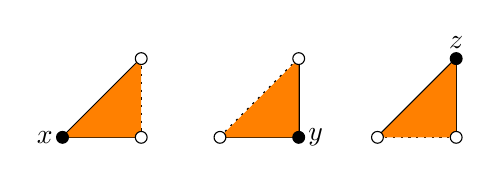
\begin{tikzpicture}
\node [left] at (0,0) {$x$};
\draw [dotted, thick] (1,1) -- (1,0);
\draw [thick] (0,0) -- (1,1);
\draw [thick] (0,0) -- (1,0);
\path [fill=orange] (0,0) -- (1,0) -- (1,1);
\draw [fill=white] ( 1,0) circle (0.075);
\draw [fill=white] ( 1,1) circle (0.075);
\draw [fill=black] ( 0,0) circle (0.075);

\node [right] at (3,0) {$y$};
\draw [thick] (3,1) -- (3,0);
\draw [dotted, thick] (2,0) -- (3,1);
\draw [thick] (2,0) -- (3,0);
\path [fill=orange] (2,0) -- (3,0) -- (3,1);
\draw [fill=black] ( 3,0) circle (0.075);
\draw [fill=white] ( 3,1) circle (0.075);
\draw [fill=white] ( 2,0) circle (0.075);

\node [above] at (5,1) {$z$};
\draw [thick] (5,1) -- (5,0);
\draw [thick] (4,0) -- (5,1);
\draw [dotted, thick] (4,0) -- (5,0);
\path [fill=orange] (4,0) -- (5,0) -- (5,1);
\draw [fill=white] ( 5,0) circle (0.075);
\draw [fill=black] ( 5,1) circle (0.075);
\draw [fill=white] ( 4,0) circle (0.075);
\end{tikzpicture}
\end{center}
The stars $x^*$ and $y^*$ share the open interior of the $1$-simplex $f$, so they glue on that piece. Moreover, they share the open interior of the $2$-simplex $(f,g)$, so the ``interiors'' are glued together too. What we are left with is the whole space minus the point $z$. So, $\ST(y) \cong X_\mathbf{C} - \{z\}$. Notice that $\ST(y) = \mu^{-1}_{\mathbf{C}}(U_y)$. For $\ST(z)$, we get the whole space $X_\mathbf{C}$. Again, $\ST(z) = \mu^{-1}_{\mathbf{C}}(U_z)$.
\end{example}

\begin{example}[The Finite Circle]
\label{ex:ST of our favorite finite space}
Take $\mathbf{C}$ to be the following poset: $a \leq c,d$, $b \leq c,d$. Then $\mathbf{C}$ may also be regarded as a finite $T_0$-space. The minimal opens are $U_a = \{a,c,d\}$, $U_b = \{b,c,d\}$, $U_c = \{c\}$ and $U_d = \{d\}$. The star sieve construction agrees with the inverse images of the McCord map.
\end{example}

\begin{example}[The Graph Category]
\label{ex:ST of the graph category}
Now it gets interesting. Take $\mathbf{C}$ to be the graph category $x \rightrightarrows y$, with $f,g : x \to y$. The realization $X_\mathbf{C}$ is a circle with two distinguished vertices $x$ and $y$. We have
\begin{align*}
\ST(x) &= x^*_{\id}, \\
\ST(y) &= x^*_f \sqcup x^*_g \sqcup y^*_{\id} / \sim.
\end{align*}
Let's compute
\begin{align*}
\st(x) &= \{x,f,g\}, \\
\st(y) &= \{y,f,g\}, \\
\st(f) &= \{f\}, \\
\st(g) &= \{g\}.
\end{align*}
Note that we leave out the degenerate simplices. 
The reader may convince himself that these are also taken care of during gluing. All possible morphisms in $\mathbf{C}/y$ are
\[ \begin{tikzcd}
x \arrow{r}{f} \arrow[swap]{dr}{f} & y \arrow{d}{\id} & x \arrow{r}{g} \arrow[swap]{dr}{g} & y \arrow{d}{\id} \\
& y & & y
\end{tikzcd}\]
Here, the open interior of the $1$-simplex $f$ is shared by the first copy $x^*_f$ and $y^*_{\id}$, so they glue on their top halves. The open interior of the $1$-simplex $g$ is shared by the second copy $x^*_g$ and $y^*_{\id}$, so they glue on their lower halves. What we are left with is a spiral that goes around $y$ once.
\[ \begin{tikzcd}
\ST(x) \arrow[equals]{d} & \; & \ST(y) \arrow[equals]{d} \\
\begin{tikzpicture}[tdplot_main_coords]
  
  \begin{scope}[color=black]
  \pgfplothandlerlineto
  \pgfplotfunction{\t}{-180,...,180}
       {\pgfpointxy {cos(\t)}{sin(\t)}{\t/360}} 
       \pgfusepath{stroke}
  \end{scope}

  \draw [fill=white] ( 1,0) circle (0.1);
  \draw [fill=black] (-1,0) circle (0.1);

  \node at (-1.4,0) {$x_{\id}$};

\end{tikzpicture} \arrow[shift left=1em, color=blue]{rr}{\ST(f)} \arrow[swap, shift right=1.5em, color=orange]{rr}{\ST(g)} \arrow[swap]{dr}{e_x} & \; & \begin{tikzpicture}[tdplot_main_coords]

  \begin{scope}[color=blue]
  \pgfplothandlerlineto
  \pgfplotfunction{\t}{-360,...,0}
       {\pgfpointxyz {cos(\t)}{sin(\t)}{-\t/360}} 
       \pgfusepath{stroke}
  \end{scope}

  \begin{scope}[color=orange, dashed]
  \pgfplothandlerlineto
  \pgfplotfunction{\t}{-180,...,0}
       {\pgfpointxyz {cos(\t)}{sin(\t)}{-\t/360}} 
       \pgfusepath{stroke}
  \end{scope}

  \begin{scope}[color=orange]
  \pgfplothandlerlineto
  \pgfplotfunction{\t}{0,...,130}
       {\pgfpointxyz {cos(\t)}{sin(\t)}{-\t/360}} 
       \pgfusepath{stroke}
  \end{scope}

  \begin{scope}[color=orange]
  \pgfplothandlerlineto
  \pgfplotfunction{\t}{145,...,360}
       {\pgfpointxyz {cos(\t)}{sin(\t)}{-\t/360}} 
       \pgfusepath{stroke}
  \end{scope}

  \begin{scope}[color=black, dashed]
  \pgfplothandlerlineto
  \pgfplotfunction{\t}{0,...,130}
       {\pgfpointxyz {cos(\t)}{sin(\t)}{-\t/360}} 
       \pgfusepath{stroke}
  \end{scope}

  \begin{scope}[color=black, dashed]
  \pgfplothandlerlineto
  \pgfplotfunction{\t}{145,...,180}
       {\pgfpointxyz {cos(\t)}{sin(\t)}{-\t/360}} 
       \pgfusepath{stroke}
  \end{scope}

  \draw [fill=black] ( 1,  0  ) circle (0.1);
  \draw [fill=black] (-1,  1  ) circle (0.1);
  \draw [fill=black] (-1, -1  ) circle (0.1);
  \draw [fill=white] ( 1, -1.8) circle (0.1);
  \draw [fill=white] ( 1,  1.8) circle (0.1);

  \node at (-1.3,1) {$x_f$};
  \node at (-1.3,-1) {$x_g$};
  \node at (1.4,0) {$y_{\id}$};

\end{tikzpicture} \arrow{dl}{e_y} \\
\; & \begin{tikzpicture}[tdplot_main_coords]
  
  \begin{scope}[color=black]
  \pgfplothandlerlineto
  \pgfplotfunction{\t}{-180,...,180}
       {\pgfpointxy {cos(\t)}{sin(\t)}{\t/360}} 
       \pgfusepath{stroke}
  \end{scope}

  \draw [fill=black] ( 1,0) circle (0.1);
  \draw [fill=black] (-1,0) circle (0.1);

  \node at (-1.3,0) {$x$};
  \node at ( 1.3,0) {$y$};

\end{tikzpicture}
& \; \\
\; & X_{\mathbf{C}} \arrow[equals]{u} & \;
\end{tikzcd} \]
\end{example}

\begin{example}[The Coequalizer Category]
\label{ex:ST of the coequalizer category}
Take $\mathbf{C}$ to be the coequalizer category $x \rightrightarrows y \to z$. Denote the morphisms by $f,g : x \to y$, $h : y \to z$, $hf = hg = k$. The realization $X_\mathbf{C}$ looks like a pancake, with vertex $x$ on the left border, vertex $z$ in the middle and $y$ on the right border. We have
\begin{align*}
\ST(x) &= x^*_{\id}, \\
\ST(y) &= x^*_f \sqcup x^*_g \sqcup y^*_{\id} / \sim, \\
\ST(z) &= x^*_k \sqcup y^*_h \sqcup z^*_{\id} / \sim.
\end{align*}
Let's compute
\begin{align*}
\st(x) &= \{x,f,g,k,(h,f),(h,g)\}, \\
\st(y) &= \{y,f,g,h,(h,f),(h,g)\}, \\
\st(z) &= \{z,h,k,(h,f),(h,g)\}, \\
\st(x) \cap \st(y) &= \{f,g,(h,f),(h,g)\}, \\
\st(x) \cap \st(z) &= \{k,(h,f),(h,g)\}, \\
\st(y) \cap \st(z) &= \{h,(h,f),(h,g)\}.
\end{align*}
Note that we leave out the degenerate simplices. 
The reader may convince himself that these are also taken care of during gluing.
The open set $x^*$ is the whole space $X_\mathbf{C}$ minus the closed line segment from $y$ to $z$. That is minus the closed $1$-simplex $h$. The open set $y^*$ is the whole space minus the closed line segment from $x$ to $y$. That is minus the closed $1$-simplex $k$. The open set $z^*$ is the interior of $X_\mathbf{C}$.
All possible morphisms in $\mathbf{C}/z$ are
\[ \begin{tikzcd}
z \arrow{r}{\id} \arrow[swap]{dr}{\id} & z \arrow{d}{\id} & y \arrow{r}{h} \arrow[swap]{dr}{h} & z \arrow{d}{\id} & x \arrow{r}{f} \arrow[swap]{dr}{k} & y \arrow{d}{h} & x \arrow{r}{g} \arrow[swap]{dr}{k} & y \arrow{d}{h} \\
& z & & z & & z & & z
\end{tikzcd} \]

\begin{itemize}
	\item[$\ST(x)$] The McCord space $\ST(x)$ is the open set $x^*$, the ``pacman face''.
	\item[$\ST(y)$] The interior of the $1$-simplex $f$ is shared by the first copy $x^*_f$ and $y^*_{\id}$, so they glue there. The interior of the $2$-simplex $(f,h)$ is shared by the first copy $x^*_f$ and $y^*_{\id}$, so they glue there. The interior of the $1$-simplex $g$ is shared by the second copy $x^*_g$ and $y^*_{\id}$, so they glue there. The interior of the $2$-simplex $(g,h)$ is shared by the second copy $x^*_g$ and $y^*_{\id}$, so they glue there. What we are left with is a spiral staircase making one roundabout.
	\item [$\ST(z)$] The $2$ copies of the $2$-simplex $(f,h)$ sitting inside $\ST(y)$ are shared by the same $2$-simplex $(f,h)$ sitting inside $z^*$, so they glue. The same holds for the $2$-simplex $(g,h)$. Moreover the simplices $k$ and $h$ glue too. So we are left with the whole space $X_\mathbf{C}$.
\end{itemize}
\end{example}

\begin{example}[The Equalizer Category]
\label{ex:ST of the equalizer category}
Take $\mathbf{C}$ to be the equalizer category $x \to y \rightrightarrows z$. Denote $h : x \to y$ and $f,g : y \to z$ with $fh = gh = k$. The realization $X_\mathbf{C}$ is again a pancake, but this time $y$ is at the left border, $x$ is in the middle and $z$ is at the right border. You can also view $X_\mathbf{C}$ as a coffee-filter, where the coffee runs down to the vertex $x$. We have
\begin{align*}
\ST(x) &= x^*, \\
\ST(y) &= x^* \sqcup y^* / \sim, \\
\ST(z) &= x^* \sqcup y^*_f \sqcup y^*_g \sqcup z^* / \sim.
\end{align*}
The open set $x^*$ is the whole space $X_\mathbf{C}$ minus the border, so minus the closed $1$-simplex $f$ and minus the closed $1$-simplex $g$. The open sets $y^*$ and $z^*$ are pacman faces.

\begin{itemize}
	\item [$\ST(x)$] This is the interior $x^*$ of $X_\mathbf{C}$.
	\item [$\ST(y)$] The interior of the $2$-simplex $(h,f)$ is shared by both $x^*$ and $y^*$, so they glue there. The interior of the $2$-simplex $(h,g)$ is shared by both $x^*$ and $y^*$, so they glue there. The interior of the $1$-simplex $h$ is shared by $x^*$ and $y^*$, so they glue there. What we are left with is the whole space $X_\mathbf{C}$ minus the point $z$.
	\item [$\ST(z)$] We go over the relevant morphisms in $\mathbf{C}/z$.
	\begin{itemize}
	\item [$k : x \to z$] We have $\st(x) \cap \st(z) = \{k, (h,f), (h,g)\}$. All three of those simplices have $k$ as a face. So $x^*$ and $z^*$ glue on the interiors of those three simplices.
	\item [$f : y \to z$] We have $\st(y) \cap \st(z) = \{f, g, (h,f), (h,g)\}$. The morphism $f$ is an eventual face of $f$ and $(h,f)$, so $y^*_f$ and $z^*$ glue on the interiors of $|f|$ and $|(h,f)|$.
	\item [$g : y \to z$] We have $\st(y) \cap \st(z) = \{f, g, (h,f), (h,g)\}$. The morphism $g$ is an eventual face of $g$ and $(h,g)$. So $y^*_g$ and $z^*$ glue on the interiors of $|g|$ and $|(h,g)|$.
	\end{itemize}
	What $\ST(z)$ looks like is hard to describe. It is sort of an oreo cookie with two infinitely close boundaries which twist at one end.
\end{itemize}
\end{example}

\begin{example}[The $2$-Element Monoid Category]
\label{ST of the 2-element monoid category}
Let $M$ be the monoid $\{1,f\}$ with $f^2 = f$, regarded as a category. The set of $n$-simplices of the nerve $NM$ are $(NM)_n = M^n$. In particular, $NM$ has just one vertex, call it $\bullet$. The realization $X_M$ is something which I cannot describe easily. It may be vaguely described as a ``fat'' point. We see that
\[ \st(\bullet) = \bigsqcup_{n \geq 0} \left(NM\right)_n. \]
In the slice category $M / \bullet$, all possible morphisms are
\[ \begin{tikzcd}
\bullet \arrow[swap]{dr}{1} \arrow{r}{1} & \bullet \arrow{d}{1} & \bullet \arrow[swap]{dr}{f} \arrow{r}{f} & \bullet \arrow{d}{1} & \bullet \arrow[swap]{dr}{f} \arrow{r}{f} & \bullet \arrow{d}{f} \\
& \bullet & & \bullet & & \bullet
\end{tikzcd} \]
Now the construction of $\mu(\bullet)$ goes as follows. We have the object $\bullet \xrightarrow{1} \bullet$ in $M/\bullet$ and the object $\bullet \xrightarrow{f} \bullet$ in $M/\bullet$. The realization $\bullet_1^*$ is $X_M$. The realization $\bullet_f^*$ is also $X_M$. What parts do we glue? The only valid morphism of the possible three above is $f : \bullet_f \to \bullet_1$. In other words, every simplex $\sigma \in \st(\bullet)$ which contains $f$ is glued between the two copies of $X_M$. What remains are the ``completely degenerate'' simplices $\sigma = (1,1,\ldots,1)$. But their realizations are just a point, so $\mu(\bullet)$ is $X_M$ with a ``double vertex'', akin to the well-known real line with double origin (which is indeed etale over the real line).
\end{example}

% \begin{proposition}
% \label{prop:ST is a faithful functor}
% $\ST : \mathbf{C} \to \mathbf{LH}/X_\mathbf{C}$ is a faithful functor.
% \end{proposition}
% \begin{proof}
% \begin{color}{red} Omitted for now. Remove this? It's not used anywhere. \end{color}
% \end{proof}
% \begin{proof}
% Suppose $A$ and $B$ are two objects of $\mathbf{C}$ and take $f,g \in \Hom_\mathbf{C}(A,B)$. Suppose that $\ST(f) = \ST(g)$. This means that for all $[h,p] \in \ST(A)$, we have $[f \circ h, p] = [g \circ h, p]$ in $\ST(B)$. Take $h = \id_A$. Then $[f,p] = [g,p]$ in $\ST(B)$ for all $p \in A^*$. Without loss of generality assume that $(f,p) \rhd (g,p)$. This means that there exists a morphism $k : f \to g$ in $\mathbf{C}/B$ and an $n$-simplex $\sigma \in \st(k)$ such that $p \in \Int(\sigma)$. Now $f$ and $g$ have the same domain and codomain, so $k$ is an endomorphism of $A$. Therefore $\st(k) = \st(A)$.
% % So there exists an $n$-simplex $\sigma \in \st(D)$ such that $f$ and $g$ are eventual faces of $\sigma$. Since $f$ and $g$ have the same codomain, this must mean that they are the same $1$-simplex, so $f=g$.
% \end{proof}

\section{Flatness Conditions}

To understand $\ST$ better, we shall study its fibers (or stalks).

\begin{definition}
\label{def:support at a point}
Let $p \in X_\mathbf{C}$. We define the \emph{support} of $p$ to be the full subcategory of $\mathbf{C}$ given by
\[ \mathbf{C}(p) := \left(\begin{array}{c} A \in \mathbf{C} : p \in A^* \\ + \\ \text{morphisms from $\mathbf{C}$} \end{array} \right). \]
\end{definition}
Note that $\mathbf{C}(p)$ is not the empty category by \cref{lem:realizations of stars form an open cover}. Put a relation on $\mathbf{C}(p)$ by declaring
\[ A \leq B \iff \Hom_\mathbf{C}(A,B) \neq \emptyset, \qquad A,B \in \mathbf{C}(p). \]
Then $\leq$ is a preorder, but usually not a partial order.

\begin{lemma}
\label{lem:different characterization of the support}
Let $p \in X_{\mathbf{C}}$. Then $p \in |\sigma|$ for a unique non-degenerate $n$-simplex $\sigma \in (N\mathbf{C})_n$. The objects of the category $\mathbf{C}(p)$ consist of the vertices of this $\sigma$.
\end{lemma}
\begin{proof}
If $A \in \mathbf{C}$ is a vertex of $\sigma$, then $\sigma \in \st(A)$. So $p \in A^*$. On the other hand, suppose that $A \in \mathbf{C}(p)$. We want to show that $A$ is a vertex of $\sigma$. We know that $p \in A^*$. So $p \in \Int(\tau)$ for some $\tau \in \st(A)$ by \cref{lem:realization of the star is union of the interiors}. So $p \in |\tau|$. Let $\sigma'$ be the unique non-degenerate simplex for $\tau$. Then $|\tau| = |\sigma'|$. Then $A$ is a vertex of $\sigma'$. By uniqueness, $\sigma = \sigma'$.
\end{proof}

Observe that if $p =|A|$ for some object $A \in \mathbf{C}$, then $\mathbf{C}(p)$ consists of a single object.

\begin{lemma}
If $\mathbf{C}$ is a finite poset, then $\mathbf{C}(p)$ is totally ordered with a minimal element for all $p \in X_{\mathbf{C}}$.
\end{lemma}
\begin{proof}
Take $p \in X_{\mathbf{C}}$. Let $\sigma$ be the unique non-degenerate simplex such that $p \in |\sigma|$. By \cref{lem:different characterization of the support}, the objects of the category $\mathbf{C}(p)$ are the vertices of $\sigma$. The vertices of an $n$-simplex in $(N\mathbf{C})_n$ are totally ordered, because $\mathbf{C}$ is a poset. Since $n < \infty$, there is a minimal element.
\end{proof}

The results of \cref{ex:ST of the three category} and \cref{ex:ST of our favorite finite space} generalize to a theorem. Recall that for a finite $T_0$-space $\mathbf{C}$, the McCord map $\mu_\mathbf{C}$ is defined to be the continuous map
\[ \mu_\mathbf{C} : X_{\mathbf{C}} \to \mathbf{C}, \qquad p \mapsto \min \mathbf{C}(p). \]

\begin{theorem}
\label{thm:mccord functor generalizes the mccord map}
Let $\mathbf{C}$ be a finite $T_0$-space, or equivalently a finite poset. For each $x \in \mathbf{C}$, denote its minimal open set around $x$ by $U_x$. Then there is a natural homeomorphism
\[ \ST(x) \cong \mu_\mathbf{C}^{-1}(U_x). \]
\end{theorem}
\begin{proof}
I claim that the etale map $e_x : \ST(x) \to X_\mathbf{C}$ has a section on $\mu_\mathbf{C}^{-1}(U_x) \subset X_\mathbf{C}$. Take a point $p \in \mu_\mathbf{C}^{-1}(U_x)$. Write $M_p = \min \mathbf{C}(p)$. 
Then $M_p \in U_x$, so $M_p \leq x$. Write $u : M_p \to x$ for the unique morphism. We now have $[u,p] \in \ST(x)$. 
Define
\[ s_x : \mu_\mathbf{C}^{-1}(U_x) \to \ST(x) \]
by sending the point $p$ to $[u,p]$. The definition of $s_x$ is unambiguous, because there is only one choice for $u$. Clearly we have $e_x \circ s_x = \id_{\mu_{\mathbf{C}}^{-1}\left(U_x \right)}$. So $s_x$ is a section. We shall now prove that $s_x \circ e_x = \id_{\ST(x)}$. Take $[g,p] \in \ST(x)$ and suppose that $(s_x \circ e_x)([g,p]) = [u,p]$. We want to show that $[g,p] = [u,p]$. Note that $g : D_g \to x$ is unique. Moreover, $D_g \in \mathbf{C}(p)$, so $M_p \leq D_g$. Let $h : M_p \to D_g$ be the unique morphism. Again by uniqueness, $h \circ g = u$. We now have a morphism $h : g \to u$ in $\mathbf{C}/x$, and $(g,h) \in \st(h)$ with $p \in \Int(g,h)$. So $[g,p] = [u,g]$.
\end{proof}

Thus, we have found a generalization of the McCord map.

% \begin{lemma}
% \label{lem:support at a vertex is a one-object category}
% If $p = |A| \in X_{\mathbf{C}}$ for some $A \in \mathbf{C}$, then the only object of $\mathbf{C}(p)$ is $A$, and the only morphisms of $\mathbf{C}(p)$ are the endomorphisms of $A$.
% \end{lemma}
% \begin{proof}
% Let $B$ be an object in the support of $p$. Then $p \in B^*$, so $p \in \Int(\sigma)$ for some $\sigma \in \st(B)$. But $p = |A|$, so the only possibility is that $\sigma$ is the $0$-simplex $B$, so $B=A$.
% \end{proof}

\begin{definition}
\label{def:alexandroff cat}
We say $\mathbf{C}$ is an \emph{Alexandroff} category if for all $p \in X_{\mathbf{C}}$
\begin{enumerate}
	\item the support $\mathbf{C}(p)$ is totally ordered with a (unique) minimal element $M_p$, and
	\item for every $A \in \mathbf{C}$ and for every $[f,p] \in e_A^{-1}(p)$ there exists a unique morphism $m : M_p \to D_f$ with the property that there is an $n$-simplex $\sigma \in \st(m)$ with $p \in \Int(\sigma)$.
	 % pair $(m, \sigma)$ with $m : M_p \to D_f$ a morphism in $\mathbf{C}$ and $\sigma \in \st(M_p) \cap (D_f)$ an $n$-simplex such that $m$ is eventually a face of $\sigma$.
\end{enumerate}
\end{definition}

\begin{remark}
I chose the name ``Alexandroff category'' because a topological space is termed an ``Alexandroff space'' when every point has a minimal open neighborhood with respect to inclusion. The second property is a technical one but it is required for \cref{lem:alexandroff implies well-fibered}.
\end{remark}

% \begin{remark}
% In \cref{def:alexandroff cat}, saying that the support of a point is totally ordered with a minimal element is the same thing as saying that there are no directed cycles in the underlying graph of the category.
% \end{remark}

\begin{example}
If $\mathbf{C}$ is a finite poset, then $\mathbf{C}$ is Alexandroff. The graph category from \cref{ex:ST of the graph category} is Alexandroff. The (co)equalizer category of \cref{ex:ST of the coequalizer category} and \cref{ex:ST of the equalizer category} is Alexandroff. The category $x \leftrightarrows y$ where the two arrows are each other's inverse, is not an Alexandroff category. On the other hand, its skeleton is the trivial category, so is Alexandroff. Hence being Alexandroff is an ``evil'' notion.
\end{example}

\begin{lemma}
\label{lem:alexandroff implies trivial endomorphisms}
If $\mathbf{C}$ is Alexandroff, then for all objects $A \in \mathbf{C}$ we have $\Hom_{\mathbf{C}}(A,A) = \{\id_A\}$.
\end{lemma}
\begin{proof}
Take $A \in \mathbf{C}$ and set $p = |A| \in X_{\mathbf{C}}$. Take an element $[f,p] \in e_A^{-1}(p)$ in the fiber. Then $f : D_f \to A$ and $p \in D_f^*$. By \cref{lem:different characterization of the support}, $D_f = M_p = A$. Then since $\mathbf{C}$ is Alexandroff, $f$ is unique, so we must have $f = \id_A$.
\end{proof}
From \cref{lem:alexandroff implies trivial endomorphisms} we see that being Alexandroff and a monoid at the same time implies that $\mathbf{C}$ is the trivial category with one object and one morphism. It also shows that being Alexandroff greatly restricts the category.

\begin{definition}
\label{def:well-fibered}
We say that $\mathbf{C}$ is \emph{well-fibered} if for all $p \in X_\mathbf{C}$ there exists an object $B \in \mathbf{C}$ such that $p^* \circ \ST \cong \Hom_\mathbf{C}(B,-)$.
\end{definition}

\begin{lemma}
\label{lem:alexandroff implies well-fibered}
If $\mathbf{C}$ is Alexandroff, then it is well-fibered.
\end{lemma}
\begin{proof}
Let $p \in X_{\mathbf{C}}$. The claim is that $p^* \circ \ST \cong \Hom_{\mathbf{C}}(M_p,-)$, where $M_p$ is defined as in \cref{def:alexandroff cat}. In other words, we need to find a natural isomorphism $\alpha : p^* \circ \ST \to \Hom_{\mathbf{C}}\left(M_p,-\right)$. To that end, define $\beta : \Hom_{\mathbf{C}}\left( M_p, - \right) \to p^* \circ \ST$ as follows. For each component $A \in \mathbf{C}$, we set 
\[ \beta_A : \Hom_{\mathbf{C}}\left(M_p,A \right) \to e^{-1}_A\left(p \right), \qquad h \mapsto [h,p]. \]
Then naturality of $\beta$ is clear. The natural transformation $\beta$ will be the inverse for the natural transformation $\alpha$. For the natural transformation $\alpha$, define it as follows.

% such that for every morphism $f : A \to B$ in $\mathbf{C}$ we have a commutative diagram
% \[ \begin{tikzcd}
% \left[ g,p \right] \arrow[mapsto]{d} & e_A^{-1}(p) \arrow{r}{\alpha_A} \arrow{d} & \Hom_\mathbf{C}(M_p, A) \arrow{d} & h \arrow[mapsto]{d} \\
% \left[ f \circ g, p \right]  & e_B^{-1}(p) \arrow{r}{\alpha_B} & \Hom_\mathbf{C}(M_p, B) & f \circ h
% \end{tikzcd} \]
Take $[g,p] \in e^{-1}_A(p)$. 
Then $g : D_g \to A$ and $p \in D_g^*$. 
So $D_g \in \mathbf{C}(p)$. Since $\mathbf{C}$ is Alexandroff, there exists a unique morphism $m : M_p \to D_g$ with the property that there is some $\sigma \in \st(m)$ such that $p \in \Int(\sigma)$. For each component $A \in \mathbf{C}$, we set
\[ \alpha_A : e^{-1}_A(p) \to \Hom_{\mathbf{C}}\left(M_p, A \right), \qquad [g,p] \mapsto g \circ m. \]
Because this $m$ is unique, $\alpha_A$ is well-defined. Observe now that
\[ \left(\beta_A \circ \alpha_A\right)[g,p] = [g \circ m, p]. \]
But $m$ has the property that we are also given a simplex $\sigma \in \st(m)$ such that $p \in \Int(\sigma)$. That means that $(g \circ m,p) \rhd (g,p)$, so $[g \circ m,p] = [g,p]$. In the other direction we find
\[ \left(\alpha_A \circ \beta_A \right)(h) = h, \]
so we conclude that $\alpha$ and $\beta$ are each other's inverse transformations.
% So every element in the fiber $e_A^{-1}(p)$ may be represented, in a unique way, as $[h,p]$ with $h : M_p \to A$ and $p \in M_p^*$. Define $\alpha_A : e^{-1}(p) \to \Hom_{\mathbf{C}}(M_p,A)$ by $[h,p] \mapsto h$. If $h = h'$, then $[h,p] = [h',p]$, and if $h \in \Hom_{\mathbf{C}}(M_p,A)$, then $[h,p] \in e^{-1}_A(p)$. So $\alpha_A$ is a bijection. If $f : A \to B$ is a morphism in $\mathbf{C}$ and $[h,p] \in e_A^{-1}(p)$, then
% \[ \alpha_B \left( [f \circ h, p] \right) = f \circ h = f \circ \alpha_A \left( [h, p] \right), \]
% so $\alpha$ is a natural isomorphism.
\end{proof}

\begin{lemma}
\label{lem:has enough points}
The topos $\mathbf{LH}/X_\mathbf{C}$ has enough points.
\end{lemma}
\begin{proof}
$X_\mathbf{C}$ is a geometric realization of a simplicial set, so $X_\mathbf{C}$ is a CW-complex by \cite[Proposition I.2.3]{goersjardinne09}. In particular it is a compactly generated Hausdorff space, and Hausdorff spaces always have enough points.
\end{proof}

Recall from \cref{def:set valued flat functor} that $\ST$ is flat when by definition the induced functor $- \otimes_{\mathbf{C}} \ST$ is left exact.

\begin{lemma}
\label{lem:well-fibered implies flat}
If $\mathbf{C}$ is well-fibered, then $\mu : \mathbf{C} \to \mathbf{LH}/X_{\mathbf{C}}$ is flat.
\end{lemma}
\begin{proof}
By \cref{lem:has enough points}, it suffices to prove that for every $p \in X_{\mathbf{C}}$ the functor $p^* \circ \mu : \mathbf{C} \to \mathbf{Set}$ is flat. This is the same thing as proving that the category of elements $\int_{\mathbf{C}} \left( p^* \circ \mu \right)$ is filtered, by \cref{thm:flat iff filtering}. Since $\mathbf{C}$ is well-fibered, there exists some object $B \in \mathbf{C}$ such that $p^* \circ \mu \cong \Hom_{\mathbf{C}}\left(B,-\right)$. Therefore,
\[ \int_\mathbf{C} \left( p^* \circ \mu \right) \cong \int_{\mathbf{C}} \Hom_{\mathbf{C}}\left(B, - \right) \cong B \backslash \mathbf{C}. \]
Now the over-category $B \backslash \mathbf{C}$ is always filtered, because $\id_B : B \to B$ is an initial object.
\end{proof}

So we see that when $\mathbf{C}$ is Alexandroff, $\mu$ is flat.

\begin{lemma}
Assume that $\mathbf{C}$ is a monoid (so consists of a single object). Let $p \in X_{\mathbf{C}}$. Denote the unique object of $\mathbf{C}$ by $\bullet$. Let $e_\bullet : \mu(\bullet) \to X_\mathbf{C}$ be the etale space of $\bullet$.
\begin{enumerate}
	\item If $p = |\bullet|$, then $e_\bullet^{-1}(|\bullet|) \cong \Hom_\mathbf{C}(\bullet, \bullet)$.
	\item If $p \neq |\bullet|$, then $e_\bullet^{-1}(p)$ is a one-element set.
\end{enumerate}
\end{lemma}
\begin{proof}
Follows from the definition of $\ST(\bullet)$.
\end{proof}

We'll end this section with a conjecture.

\begin{conjecture}
\label{conj:if C is a monoid then ST is flat}
If $\mathbf{C}$ is a monoid, then $\mu : \mathbf{C} \to \mathbf{LH}/X_{\mathbf{C}}$ is flat.
\end{conjecture}

The evidence lies in the fact that $X_\mathbf{C}$ may be regarded as the classifying space of the monoid $\mathbf{C}$, so its fundamental group is the groupification of $\mathbf{C}$ (for instance, see \cite{lenz2011}). Moreover, the fundamental group of the presheaf topos on $\mathbf{C}$ is (the profinite completion of) the groupification of $\mathbf{C}$. So in this sense, the McCord functor $\ST$ should detect that.